\clearpage
\section{Dynamic Time Warping}
\label{dtw}

Now that there are representative models of all time series, the issue at hand is
how to compare these models. Dynamic time warping
is a method for computing the distance between any two time series. The time 
series need not be of the same length.  Furthermore, the time series may be 
decomposed into a set of representative spectra and the DTW may still be applied.
The distance computed by DTW is a measure of the changes that would need to be 
made to one time series to turn it into (warp) the other time series. Thus, 
the DTW distance is a measure over the whole time series, and not just a 
single characteristic point. As with Gaussian processes, a number of more thorough
resources, such as \cite{muller}, cover dynamic time warping in greater detail.
Here a minimal introduction is given that enables meaningful figure-of-merit 
calculations.

With respect to nuclear fuel cycle benchmarks, there are two main DTW applications.
The first is to compute the distance between a Gaussian process model and each of 
the simulators that made up the training set for that model. This gives a 
quantitative measure 
of how far each simulator is from the model and can help determine which 
simulators are outliers. To maintain a non-judgmental benchmark, though, it is 
critical to not then use this information to discard outliers.  Rather, outlier
identification should be used as part of an inter-code comparison. If one simulator
is an outlier for a given metric, the reasons for this should be investigated. 
For example, the outlier simulator may be at a higher fidelity level, there may be 
a bug in the outlier, or there may be a bug in all other simulators. Identifying 
outliers for many metrics could help discover the underlying cause of any 
discrepancies.

The second application of dynamic time warping to benchmarking is to compare 
the constituent 
feature models to the total model.  Distances computed in this manner allow 
for a rank ordering of the components.  This enables the benchmark to make claims
about which features drive the fuel cycle metric most strongly over the whole 
simulation time domain and for all simulators. Traditionally, the simulators have 
to agree
within nominal error bounds ($<5\%$) for a benchmark to make such a claim.  Here,
the simulators need not necessarily agree since the Gaussian process models are
used as representatives.  In this application, it is useful to recast the DTW 
distance as a measure of contribution.  Contribution FOMs will be presented in 
\S\ref{contribution}.

For any two time series, dynamic time warping consists of three mathematical objects:
the distance $d$, a cost matrix $C$, and a warp path $w$. The cost matrix 
specifies how far a point on the first time series is from another point on the 
other time series.  The warp path is then the minimal cost curve through this 
matrix from the fist point in time to the last. The distance, therefore, is the
total cost of traversing the warp path.

The first step in a dynamic time warping algorithm is to compute the cost matrix. 
Suppose that the first 
time series $x$ has length $A$ indexed by $a$ and the second time series $y$ has 
length $B$ indexed by $b$. It is helpful to define an $A\times B$ matrix $\Delta L$
that is the $L_1$ norm of the difference of time series $x$ and $y$:
\begin{equation}
\label{delta-l1}
\Delta L_{a,b} = \left|x_a - y_b\right|_1
\end{equation}
The cost matrix $C$ is then an $A\times B$ sized matrix that is defined by the 
following recursion relations:
\begin{equation}
\label{cost-matrix}
\begin{split}
C_{1,1} & = \Delta L_{1,1}\\
C_{1,b+1} & = \Delta L_{1,b} + C_{1,b}\\
C_{a+1,1} & = \Delta L_{a,1} + C_{a,1}\\
C_{a+1,b+1} & = \Delta L_{a,b} + \min\left[C_{a,b}, C_{a+1,b}, C_{a,b+1}\right]
\end{split}
\end{equation}
The boundary conditions in Equation \ref{cost-matrix} are equivalent 
to applying an infinite cost to any $a$ or $b$ less than or equal to zero.
The units of the cost matrix are the same as the units of the metric. However, the 
scale of the cost matrix is geometrically larger than the metric itself. This is
due to the compounding nature of the recursive definition of $C$.

Given $C$, the warp path is thus a sequence of coordinate points that can then be 
computed by traversing backwards through the matrix from $(A, B)$ to $(1, 1)$.
For a point $w_p$ in the warp path, the previous point $w_{p-1}$ is given by 
where the cost is minimized among the locations one column over $(a,b-1)$, 
one row over $(a-1,b)$, and one previous diagonal element to $(a-1,b-1)$. 
Symbolically, 
\begin{equation}
\label{warp-path}
w_{p-1} = \argmin\left[C_{a-1,b-1}, C_{a-1,b}, C_{a,b-1}\right]
\end{equation}
The maximum possible length of $w$ is thus $A + B$ and the minimum length is 
$\sqrt{A^2 + B^2}$. The warp path itself could potentially serve as a FOM.  
However, doing so would not take into account the cost along this path.

Therefore, the distance $d$ is defined as a FOM which does include for the cost of the
warp.  Due to the recursion relations used to define the cost matrix, $d$ can be 
stated succinctly as:
\begin{equation}
\label{d-calc}
d = \frac{C_{A,B}}{A + B}
\end{equation}
That is, $d$ is the final value of the cost matrix divided by the maximal length 
of the warp path. When $d$ is zero, this indicates that the two time series
are excatly the same. Thus small, positive values of $d$ suggest that the 
time series are similar to one another while larger values denote that they 
are distinct. The magnitude of large and small is dependent on the range of 
the time series. A simple definition of large is the maximum 
value of either of the time series times the length of the time series, 
while small is a representative fraction of this (e.g. 1\%, 5\%, or similiar).

For all practical purposes in nuclear fuel cycle benchmarking, $A$ and $B$ can be 
forced to have the same
value. This is because the Gaussian process model can be used to predict a time series 
with whatever time grid is desired.  The advantage of using a regression model 
is that it allows the analyst to force the same time grid.  The advantage of 
dynamic time warping is that ensuring the same time grid is not necessary.
Coupling Gaussian processes and DTW together is a more robust analysis tool 
than the methods individually.

\begin{figure}[htb]
\centering
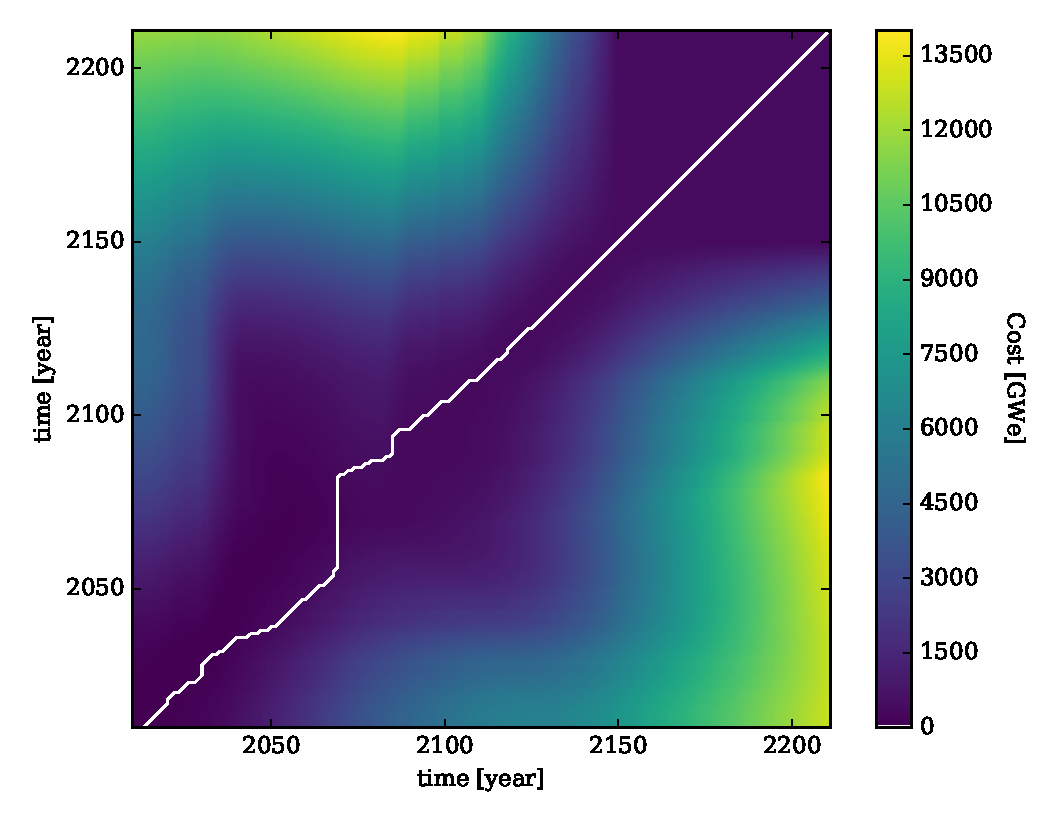
\includegraphics[width=0.9\textwidth]{cost-lwr-model-to-lwr-cyclus.eps}
\caption{Heat map of the cost matrix between the Gaussian process model 
for LWRs, $m_*^\LWR(t)$, and the Cyclus LWR time series, $m_\CYCLUS^\LWR(t)$.
The warp path is superimposed as the white curve on top of the cost matrix.}
\label{cost-lwr-model-to-lwr-cyclus}
\end{figure}

Figure \ref{cost-lwr-model-to-lwr-cyclus} displays an example cost matrix 
as a heat map for the DTW between the LWR Gaussian process model 
$m_*^\LWR(t)$ and the original Cyclus LWR time series $m_\CYCLUS^\LWR(t)$.
Additionally, the warp path between these two is shown as the white curve
on top of the heat map. Note that while $w$ is monotonic along both time axes, the
path it takes minimizes the cost matrix at every step. Higher cost regions,
seen as the brighter and more yellow or green areas in Figure \ref{cost-lwr-model-to-lwr-cyclus},
have the effect of pushing the warp path along one axis or another. The 
distance between these two curves $d(m_*^\LWR, m_\CYCLUS^\LWR)$ is computed 
to be 1.053 GWe. For scale, the maximum of the cost matrix divided by the 
maximum path length, or $\max[C]/(A+B)$, in this case is 34.86 GWe.  This 
indicated that that Cyclus LWR time series matches the model to within 3\%.

The process of dynamic time warping model generated data to raw simulator data can be 
repeated for all combinations of simulators and features. The 
$d(m_*^i, m_s^i)$ that are computed may then directly serve as a FOM for
outlier identification. Only distances between the same feature $i$ may be compared,
as they share the same model. For instance, it is valid to compare
$d(m_*^\LWR, m_\DYMOND^\LWR)$ and $d(m_*^\LWR, m_\CYCLUS^\LWR)$. However,  
it is not valid to compare $d(m_*^\LWR, m_\DYMOND^\LWR)$ and 
$d(m_*^\FR, m_\DYMOND^\FR)$.  In the situation, where the simulators 
have different time grids, the model can be evaluated with each time grid
prior to computing the corresponding DTW distances and the comparison will
remain valid.

\begin{table}[htb]
\centering
\caption{Distances [GWe] between models and simulators for all combinations of 
simulators (DYMOND and Cyclus) and metric features (generated power for 
LWRs, FRs, and in total). The simulators are presented in the rows and the
features are given as columns. Distances, as computed by 
Equation \ref{d-calc}, may only be compared along each column.}
\label{d-compare}
\begin{tabular}{l||c||c||c|}
                & \textbf{LWR} & \textbf{FR} & \textbf{Total} \\
\hline
\textbf{DYMOND} & 1.452        & 2.783       & 3.022          \\
\hline
\textbf{Cyclus} & 1.053        & 3.732       & 3.984          \\
\hline
\end{tabular}
\end{table}

Table \ref{d-compare} gives the distances for all simulator and feature 
combinations in the sample data presented in \S\ref{setup}. Only the differences between DYMOND and 
Cyclus for the same feature may be directly compared.  However, Table \ref{d-compare} 
does indicate that the DYMOND is closer to the model since both the FR and total
generated power distances are closer for DYMOND than for Cyclus.  As many
simulators as desired could be added to the benchmark and distances could 
be tallied for them as well. At a sufficient number of simulators, usual 
statistics (mean, standard deviation) along each column may be computed.
Simulators whose metrics fall outside of a typical threshold of the mean
(one or two standard deviations) would then be considered outliers and 
subject to further inter-code comparison. The two simulators here are 
for demonstration purposes and neither can be said to be an outlier in a
non-judgmental way. Recall, though, that outliers determined in this way 
may stem from the more correct simulator. The term outlier is not a 
condemnation on its own.

The second application of DTW to nuclear fuel cycle benchmarking is as a
FOM for contribution of constituent features to a total metric. For this application, 
compute the distance between the model of the total and the model of the 
part, namely $d(m_*^\Total, m_*^i)$ for all $i \in I$. This provides a 
measure of how much the total metric is determined by a particular part
over the whole time series for all simulators.
Using this measure is only reasonable if the total metric is known 
to be the sum of its constituents.  This assumption is valid for 
a large percentage of nominal benchmarking metrics. In particular, 
mass flows and generated power both follow this rule. Metrics that are 
linear transformations of these basic metrics (such as decay heat or 
radiotoxicity) will also conform to this constraint. The distances computed here
can then be used to rank order the importance of each constituent feature. 
Smaller distances are closer to the total and thus have a greater impact.

In the sample data here, the total generated power model can be compared to 
the models for LWR and FR generated power. The value of 
$d(m_*^\Total, m_*^\LWR) = 97.010$ while $d(m_*^\Total, m_*^\FR) = 19.503$.
These two values represent a comparsion of a partition of a total metric, 
as described above.  Furthermore, since this is a comparison of models and not
of simulators, this comparison is non-judgemental with resepect to the 
simulators that comprise the models. Therefore, the any claims about the
impact of different constiteunts of the partition (LWRs vs FRs) is more general
than if the impact had been measured only with a single smulator.
As expected, because this is a 1\% growth scenario, the FRs are a more 
important driver of the transition system (lower $d$ value) than the 
LWRs (higher $d$ value) over the time domain examined. Alternatively, if this
were a decrease scenario (i.e. negative growth)
that retained transition, it is not clear whether LWRs or FRs would 
provide a greater impact to the total power generated. The method detailed
here, though, grants a mechanism for comparing models in all potential 
scenarios. Figures 
\ref{cost-total-model-to-lwr-model} \& \ref{cost-total-model-to-fr-model}
show the cost matrices and warp paths for these two cases.  Notice that in the
FR case, the warp path is effectively flat until the FRs are deployed in 
significant numbers. 
 
\begin{figure}[htb]
\centering
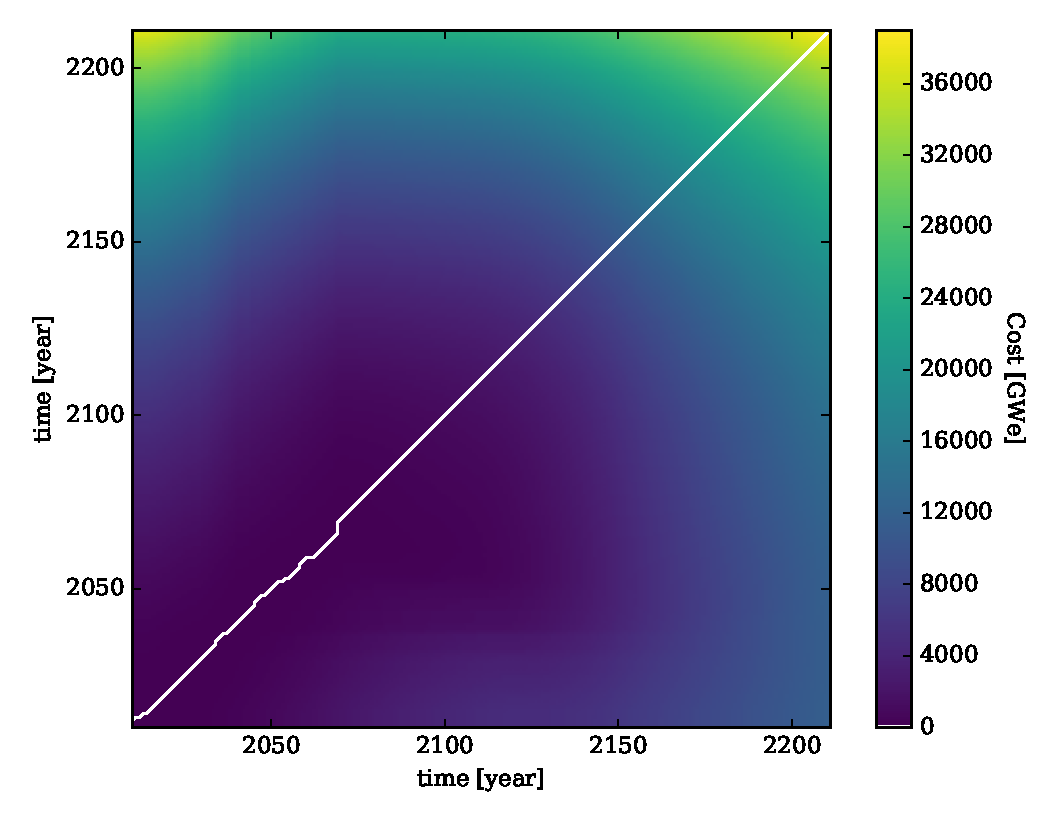
\includegraphics[width=0.9\textwidth]{cost-total-model-to-lwr-model.eps}
\caption{Heat map of the cost matrix between the Gaussian process model 
for total generated power, $m_*^\Total(t)$, and the LWR model, 
$m_*^\LWR(t)$.
The warp path is superimposed as the white curve on top of the cost matrix.}
\label{cost-total-model-to-lwr-model}
\end{figure}

\begin{figure}[htb]
\centering
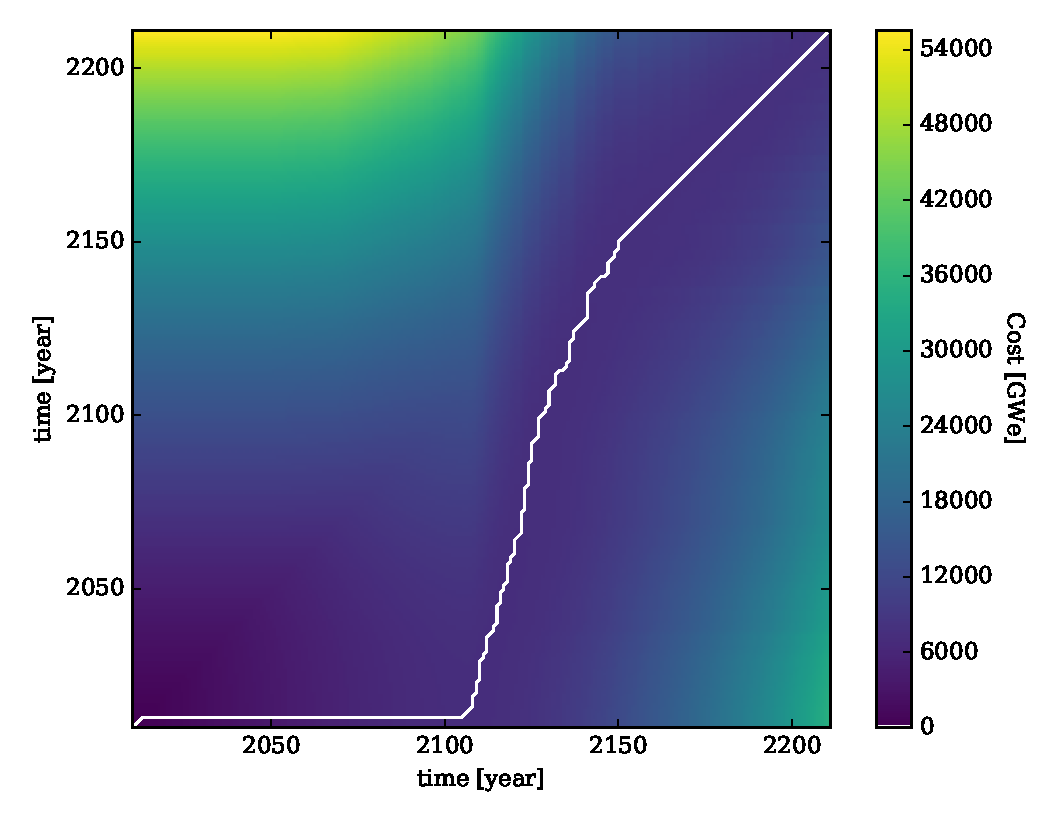
\includegraphics[width=0.9\textwidth]{cost-total-model-to-fr-model.eps}
\caption{Heat map of the cost matrix between the Gaussian process model 
for total generated power, $m_*^\Total(t)$, and the FR model, 
$m_*^\FR(t)$.
The warp path is superimposed as the white curve on top of the cost matrix.}
\label{cost-total-model-to-fr-model}
\end{figure}

In summary, dynamic time warping yields a meaningful mechanism for benchmarks to 
compare various simulators and models. As a tool for
outlier identification, it allows for each simulator to use its own native 
time grid. As a tool for performing rank ordering of features, the DTW distances
are a perfectly functional FOM. However, lower distances implying higher 
importance may run counter to intuition. The potential for confusion, therefore,
makes it less than ideal as a FOM on its own. A remedy for this is presented
in the next section in form of a new contribution FOM.
